%% This is file `elsarticle-template-1-num.tex',
%%
%% Copyright 2009 Elsevier Ltd
%%
%% This file is part of the 'Elsarticle Bundle'.
%% ---------------------------------------------
%%
%% It may be distributed under the conditions of the LaTeX Project Public
%% License, either version 1.2 of this license or (at your option) any
%% later version.  The latest version of this license is in
%%    http://www.latex-project.org/lppl.txt
%% and version 1.2 or later is part of all distributions of LaTeX
%% version 1999/12/01 or later.
%%
%% The list of all files belonging to the 'Elsarticle Bundle' is
%% given in the file `manifest.txt'.
%%
%% Template article for Elsevier's document class `elsarticle'
%% with numbered style bibliographic references
%%
%% $Id: elsarticle-template-1-num.tex 149 2009-10-08 05:01:15Z rishi $
%% $URL: http://lenova.river-valley.com/svn/elsbst/trunk/elsarticle-template-1-num.tex $
%%
\documentclass[preprint,12pt]{elsarticle}

%% Use the option review to obtain double line spacing
%% \documentclass[preprint,review,12pt]{elsarticle}

%% Use the options 1p,twocolumn; 3p; 3p,twocolumn; 5p; or 5p,twocolumn
%% for a journal layout:
%% \documentclass[final,1p,times]{elsarticle}
%%\documentclass[final,1p,times,twocolumn]{elsarticle}
%% \documentclass[final,3p,times]{elsarticle}
%% \documentclass[final,3p,times,twocolumn]{elsarticle}
%% \documentclass[final,5p,times]{elsarticle}
%% \documentclass[final,5p,times,twocolumn]{elsarticle}

%% if you use PostScript figures in your article
%% use the graphics package for simple commands
%% \usepackage{graphics}
%% or use the graphicx package for more complicated commands
%% \usepackage{graphicx}
%% or use the epsfig package if you prefer to use the old commands
%% \usepackage{epsfig}

%% The amssymb package provides various useful mathematical symbols
\usepackage{amssymb}
%% The amsthm package provides extended theorem environments
%% \usepackage{amsthm}

%% The lineno packages adds line numbers. Start line numbering with
%% \begin{linenumbers}, end it with \end{linenumbers}. Or switch it on
%% for the whole article with \linenumbers after \end{frontmatter}.
%% \usepackage{lineno}

%% natbib.sty is loaded by default. However, natbib options can be
%% provided with \biboptions{...} command. Following options are
%% valid:

%%   round  -  round parentheses are used (default)
%%   square -  square brackets are used   [option]
%%   curly  -  curly braces are used      {option}
%%   angle  -  angle brackets are used    <option>
%%   semicolon  -  multiple citations separated by semi-colon
%%   colon  - same as semicolon, an earlier confusion
%%   comma  -  separated by comma
%%   numbers-  selects numerical citations
%%   super  -  numerical citations as superscripts
%%   sort   -  sorts multiple citations according to order in ref. list
%%   sort&compress   -  like sort, but also compresses numerical citations
%%   compress - compresses without sorting
%%
%% \biboptions{comma,round}

% \biboptions{}

\usepackage{url}
\usepackage{graphicx}
\usepackage{verbatim}
\usepackage{multirow}
\usepackage{rotating}
\usepackage{moreverb}                    % for boxedboxedverbatim
\usepackage{array}
\usepackage{fancyvrb}
\usepackage{multicol}
\usepackage{mdwlist}
\usepackage{enumerate}
\usepackage{caption}
\usepackage{fancyvrb}
\usepackage{verbatim}
\usepackage{listings}
\usepackage[usenames,dvipsnames,svgnames,table]{xcolor}

\renewcommand{\theFancyVerbLine}{%
\textcolor{Black}{\scriptsize%
\arabic{FancyVerbLine}.}}

\newenvironment{mylisting}
{\begin{list}{}{\setlength{\leftmargin}{1em}}\item\small}
{\end{list}}

\newenvironment{mytinylisting}
{\begin{list}{}{\setlength{\leftmargin}{1em}}\item\tiny\bfseries}
{\end{list}}
%% \usepackage{listings} %% Break lines within verbatim

\journal{Advanced Engineering Informatics}

\begin{document}

\begin{frontmatter}

%% Title, authors and addresses

%% use the tnoteref command within \title for footnotes;
%% use the tnotetext command for the associated footnote;
%% use the fnref command within \author or \address for footnotes;
%% use the fntext command for the associated footnote;
%% use the corref command within \author for corresponding author footnotes;
%% use the cortext command for the associated footnote;
%% use the ead command for the email address,
%% and the form \ead[url] for the home page:
%%
%% \title{Title\tnoteref{label1}}
%% \tnotetext[label1]{}
%% \author{Name\corref{cor1}\fnref{label2}}
%% \ead{email address}
%% \ead[url]{home page}
%% \fntext[label2]{}
%% \cortext[cor1]{}
%% \address{Address\fnref{label3}}
%% \fntext[label3]{}

\title{Software Tools for XML to OWL Translation}

%% use optional labels to link authors explicitly to addresses:
%% \author[label1,label2]{<author name>}
%% \address[label1]{<address>}
%% \address[label2]{<address>}

\author{Thomas R. Kramer, \corref{TRK} Benjamin H. Marks, \corref{BHM}
  Craig Schlenoff, \corref {CS} Stephen Balakirsky, \corref{SB} Zeid
  Kootbally, \corref{ZK} Anthony Pietromartire \corref{AP} }

\cortext[TRK]{T. R. Kramer is a guest researcher at the National Institute
  of Standards and Technology, Gaithersburg, MD 20899 USA (e-mail:
  kramer@nist.gov).}
\cortext[BHM]{B. H. Marks is a student at Swarthmore College,
  Swarthmore, PA 19081 USA (e-mail: bmarks1@swarthmore.edu).}
\cortext[CS]{C. Schlenoff is with the National Institute of Standards and
  Technology, Gaithersburg, MD 20899 USA (e-mail: craig.schlenoff@nist.gov).}
\cortext[SB]{S. Balakirsky is with the Georgia Tech Research Institute,
  Atlanta, GA 20899 USA (e-mail: stephen.balakirsky@gtri.gatech.edu). }
\cortext[ZK]{Z. Kootbally is a guest researcher at the National Institute
  of Standards and Technology, Gaithersburg, MD 20899 USA (e-mail:
  zeid.kootbally@nist.gov). }
\cortext[AP]{A. Pietromartire is a guest researcher at the National
  Institute of Standards and Technology, Gaithersburg, MD 20899 USA (e-mail:
  pietromartire@nist.gov). }


\address{National Institute of Standards and Technology
		Gaithersburg, MD 20899, USA}



\begin{abstract}
%% Text of abstract
This paper describes a set of closely related C++ software tools for
manipulating XML schemas and XML instance files and translating them into
OWL class files and OWL instance files: (1) an XML schema parser (2) an XML
instance file parser generator, (3) the instance file parsers generated by
generator 2, (4) an XML schema to OWL class generator, (5) a domain
instance XML to OWL translator generator, and (6) the domain instance XML
to OWL translators generated by generator 5. These tools have been applied
to information models for kitting environments and kitting plans. The main
focus is on the last three tools, which differ significantly from existing
resources. The tools were built at the National Institute of Standards and
Technology in support of the Knowledge Driven Planning and Modeling project
conducted in connection with the Working Group on Ontologies for Robotics
and Automation of the IEEE Robotics and Automation Society.
\end{abstract}

\begin{keyword}
%% keywords here, in the form: keyword \sep keyword
automatic \sep C++ \sep information model \sep generator \sep ontology \sep OWL \sep schema \sep software \sep tool \sep translator \sep XML\sep XSDL
%% MSC codes here, in the form: \MSC code \sep code
%% or \MSC[2008] code \sep code (2000 is the default)

\end{keyword}

\end{frontmatter}

% \linenumbers

%% main text
\section{Introduction}
\label{}

The IEEE Robotics and Automation Society's Ontologies for Robotics
and Automation (ORA) Working Group is dedicated to developing a knowledge
representation for robotics and automation. As part of this working group,
the Industrial Robots sub-group is tasked with studying industrial
applications of the knowledge representation. One of the first areas of
interest for this subgroup is the area of kit building or kitting. This is
a process that brings parts that will be used in assembly operations
together in a kit and then moves the kit to the area where the parts are
used in the final assembly. It is anticipated that utilization of the
knowledge representation will allow for the development of higher
performing kitting systems. The Knowledge Driven Planning and Modeling
project at the National Institute of Standards and Technology worked in
collaboration with the ORA group to develop information models related to
kitting, including a model of the kitting environment and a model of a
kitting plan.

Early in its existence, the ORA group made a commitment to use OWL (Web
Ontology Language) for its models. As the authors used OWL, difficulties
arose as described in section \ref{xsdlAndOWL}. The nature of the models
being built lent itself to a more structured object model approach of the
sort used in languages such as EXPRESS \cite{express}, C++ classes \cite{c++}, and XML Schema Definition Language (XSDL)
\cite{xmlSchema0,xmlSchema1,xmlSchema2,definitive}. It was decided to use XSDL as the language for
initial modeling in the KDPM project and to produce OWL models from the
XSDL models. One author had already had experience with XSDL and was
building C++ software tools for manipulating XML schemas and instance
files. To make the translation work easier and more reliable, additional
C++ tools were built for that purpose.

Much research has been devoted to translating XML into OWL. A
comparison between existing utilities can be found in \cite{albarrak,bedini,yahia}. Nevertheless, existing software has many
limitations. In some cases, the software converts only XML Schema \cite{tsinaraki} or requires an existing OWL ontology \cite{rodriguez}. The majority of tools incorporate information
from either XML schema files or XML instance files, but not both \cite{bohring,garcia,ghawi}.  This
precludes the creation of accurate OWL instances from XML instances
that conform to an XML schema.  Additionally, existing utilities do
not scale well with input size or complexity, either requiring human
verification and restructuring of the converted file \cite{ghawi}
or limiting the potential complexity of XML schema files by only
analyzing a single schema at a time \cite{garcia}. Finally, most
tools are implemented using mappings encoded in XML stylesheets \cite{thuy,yahia,ontmalizer}, which
seem to scale in exponential time with the length of the converted
document \cite{bohring}.  For all of these reasons, a different,
scalable approach is needed.

The remainder of this paper focuses on the tools and how the translation
tools were tailored to deal with the differences between OWL and XSDL.
Section II describes the tools. Section III describes key differences
between XSDL and OWL. Section IV gives details about the software in the
tools, and Section V presents conclusions and future work.

Reserved words from XSDL and OWL or from sample files are set {\tt in
  this font}.

\section{The Tools}
\label{tools}

Figure \ref{flowchart} shows the tools, the file types the tools
manipulate, and the connections among them. The tools all run from a
command window; they have no graphical user interfaces. This makes them
independent of any operating system.

\begin{figure}
	\centering
	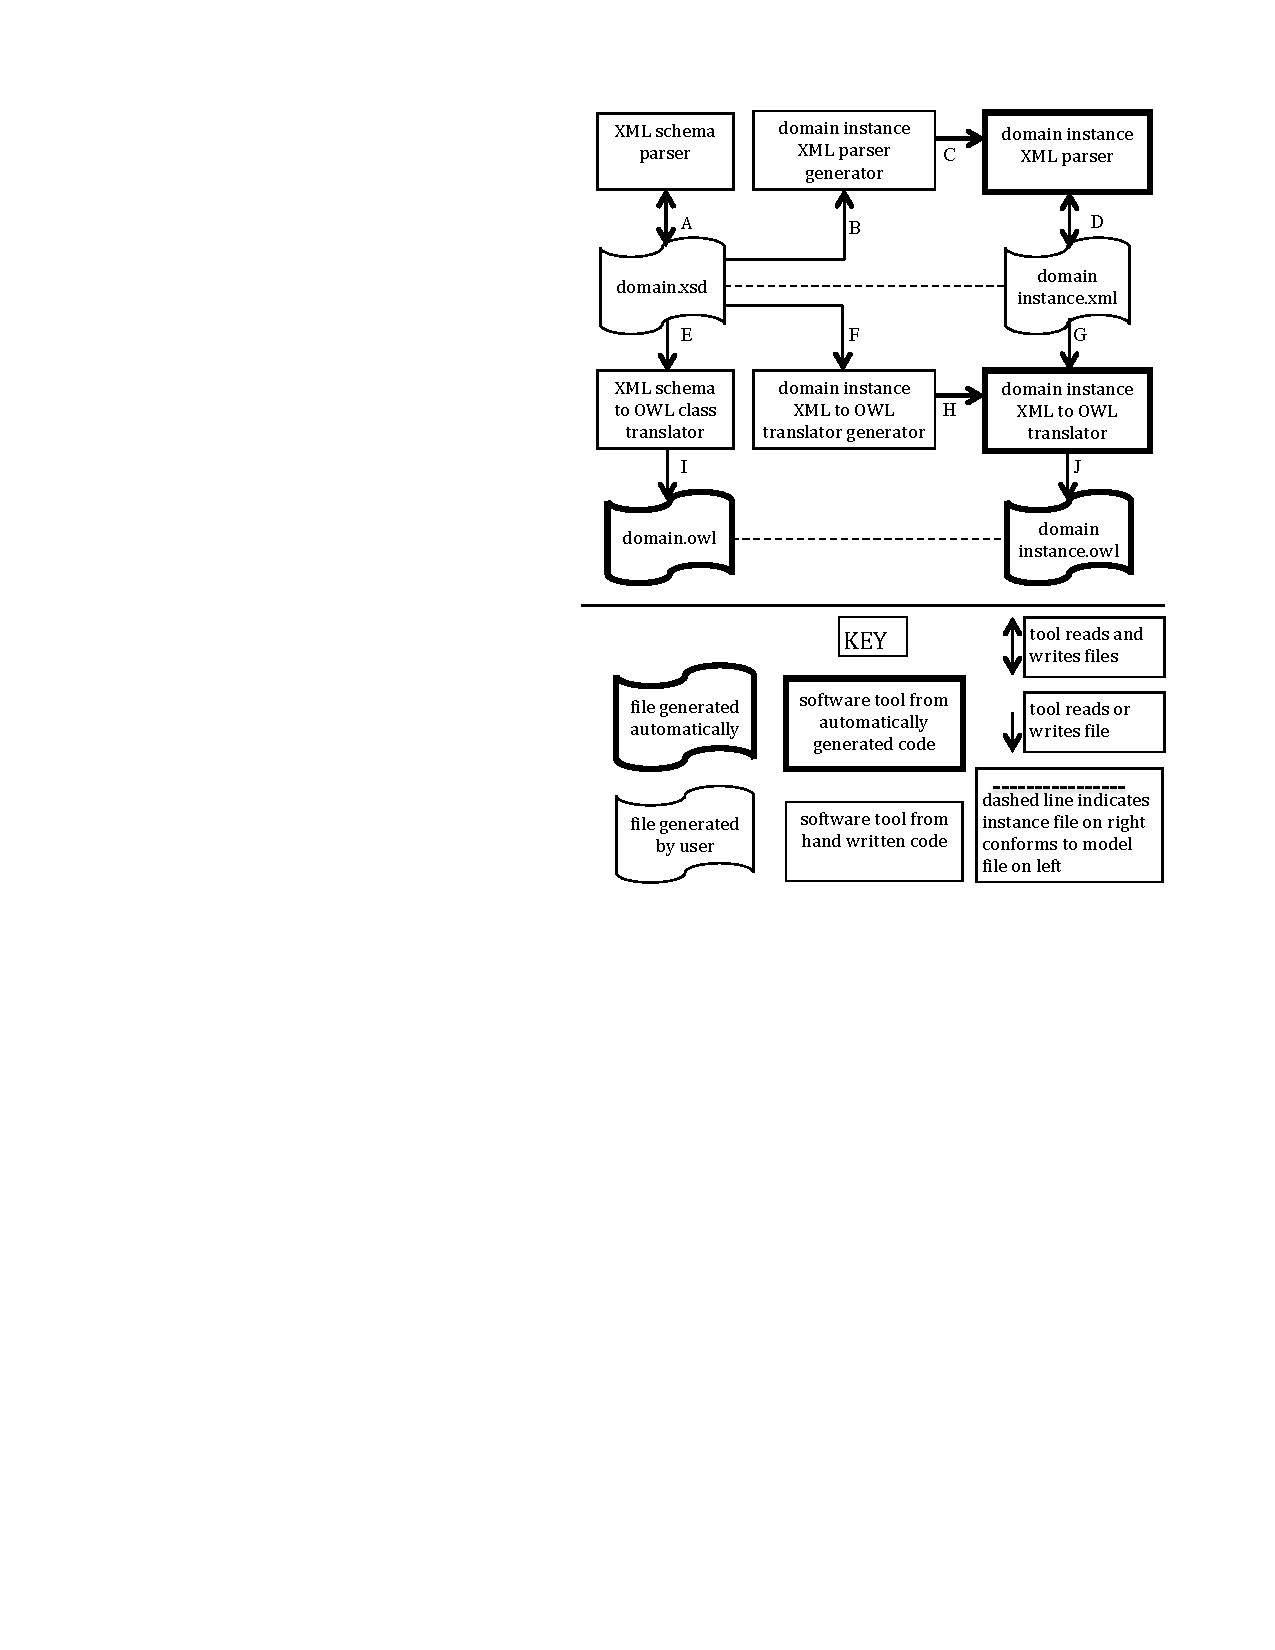
\includegraphics [width=0.8 \textwidth]{ConversionChart.pdf}
	\caption{Software Tools, Model Files, and Instance Files}
	\label{flowchart}
\end{figure}

The files (domain.xsd and domain.owl) on the left side are information
model files. They show how instances of information should be structured.
For example, a point might be modeled in an information model as x, y, and
z coordinate values. The files on the right side (domain-instance.xml and
domain-instance.owl) are instance files that contain specific data
instances that conform to an information model. For example, a specific
point in an instance file might be (1, 2, 3), corresponding to the x, y, z
model. Many instance files may correspond to a given information model.

The subject matter area of an information model is called its domain. The
tools on the left and in the middle of Figure \ref{flowchart} are domain
independent. Each tool will work with any XML {\tt schema} that meets that
tool's restrictions on the usage of the XSDL. The restrictions vary among
the tools. The tools on the right side of the figure are domain dependent.
They take as input only XML instance files in the domain for which the
tools were generated.

\subsection{XML Schema Parser}
\label{schemaParser}

As indicated by arrow A on Figure \ref{flowchart}, the XML schema parser
(henceforth xmlSchemaParser) reads and writes XML {\tt schema} files. It is
able to handle almost all of XSDL. When it runs, it reads an input file,
stores it in terms of a C++ class model of XSDL {\tt schema}s, and reprints
it in a file with almost the same name as the input file; ``echo'' is
appended to the file name. The output file is formatted to be easily human
readable for the few humans who read XSDL files directly. While it runs,
the xmlSchemaParser prints what it is reading in the command window in
which it is running. If there is any syntax error, the xmlSchemaParser
stops reading at the point where the first error occurred, prints an error
message, and exits; no output file is generated.

In comparison with commercially available tools, and good free tools, this
xmlSchemaParser has few advantages for general use. However, since it uses
a YACC-Lex parser, it is very fast. It runs in $\mathcal{O}{(N)}$ time
where ${N}$ is the number of lines in the {\tt schema} file. Also, it has
one set of specialized options that were developed for another project.
That is, the user has a choice of how {\tt documentation} nodes are handled
when the output file is generated. XSDL {\tt documentation} nodes may be
(1) deleted entirely, (2) formatted automatically for human readability, or
(3) printed in a single string (for input to some other automatic
formatting tool). In the second option, {\tt documentation} nodes that have
been specially formatted (as evidenced by extra indenting on one or more
lines) are not reformatted. There is another option for retaining comments
or removing them. That option has a simple implementation but requires that
comments be located in the {\tt schema} only where annotation nodes are
allowed.

\subsection{Domain Instance XML Parser Generator}
\label{parserGenerator}

The Domain Instance XML Parser Generator (henceforth
xmlInstanceParserGenerator) reads an XML {\tt schema} that models some
domain and writes software for a parser that reads and writes XML instance
files conforming to the {\tt schema}. This is indicated by arrows B and C
on Figure \ref{flowchart}. The xmlInstanceParserGenerator is by far the
most complex of the tools described in this paper. For a {\tt schema} up to
several thousand lines long, however, it runs in a fraction of a second on
an ordinary desktop or laptop computer. If the number of {\tt complexType}s
in a {\tt schema} file is ${N}$, the time taken by the
xmlInstanceParserGenerator is $\mathcal{O}{(N^2)}$.

The files that are generated from the domain.xsd XML {\tt schema} file
(where domain may be any name allowed by XSDL and C++) are:
\begin{itemize}
\item[] domain.lex –-- a Lex file for a lexical scanner used by the YACC parser.
\item[] domain.y --- a YACC file for a parser for XML files in the domain. 
\item[] domainClasses.hh --- a C++ header file defining classes for
      the domain. Each class has two constructors, a destructor, 
      and a printSelf function.
\item[] domainClasses.cc --– a C++ code file implementing the classes.
\item[] domainParser.cc --– a C++ code file with a main program.
\end{itemize}

If the XML {\tt schema} file on which the xmlInstanceParserGenerator is
operating {\tt include}s one or more other XML {\tt schema} files, a pair
of domainClasses C++ files is generated for each additional {\tt schema}
file, but there is still only one Lex file, one YACC file, and one main
program file.

After the xmlInstanceParserGenerator has finished running, further
processing builds a Domain Instance XML Parser. The flex Lex processor \cite{lexAndYacc,flex} is used to generate the C++ file
domainLex.cc automatically from domain.lex. The Bison YACC processor \cite{yacc,lexAndYacc} is used to generate domainYACC.cc
and domainYACC.hh automatically from domain.y. The four (or more) .cc files
are then compiled and linked in the usual way, i.e. by using a Makefile in
any operating system that uses standard Makefiles or by using Visual Studio
for MS Windows \cite{msC++}. As described in Section IV, an additional
object file is also linked in.

In comparison with commercially available code generation tools, and good
free tools, the xmlInstanceParserGenerator has few advantages for general
use. The principal advantage to the authors is that we understand the code
and can add any functionality we need. In addition, the many months
invested in writing the code paid off in minimizing the time it took to
build the XML Schema to OWL Class Translator, and the Domain Instance XML
to OWL Translator Generator, each of which required only a week or so.
Another, possibly minor, advantage is that all output code files are
carefully formatted to be human readable – if the reader is familiar with
the language in which the file is written.

Another useful feature of the xmlInstanceParserGenerator is the ability to
preserve changes made manually to the automatically generated
domainClasses.hh header file if the input {\tt schema} is modified and the
header file is regenerated. If the arguments to the command that starts the
xmlInstanceParserGenerator include {\em -h domainClasses.hh}, where {\em
  domainClasses.hh} is the old manually changed header file, any allowed
changes in the old header file will be transcribed into the corresponding
positions in the new header file that is generated. Two types of changes to
header files are allowed. First, immediately after the list of \#includes
near the top of the file, a // style comment line may be inserted followed
by more \#includes. Second, immediately before the right curly brace that
closes each class declaration, a // style comment line may be inserted
followed by any lines that are syntactically correct in that position (for
example, an attribute declaration or a constructor declaration). To
accomplish the transcription of the latter type of changes, when the
xmlInstanceParserGenerator starts, it reads the old header file and builds
a map from class names to lists of character arrays containing the changes.
When the new header is being printed, just before the printing of each
class ends, the map is checked and the contents of the list of changes for
that class are copied into the new header file. At the same time, ``done'' is
put at front of the list to indicate that the changes for that class have
been transcribed. After the new header file has been generated, the change
map is checked to be sure all changes are marked done. If a change is not
marked done, that implies that a class defined in the old header file is
not present in the new one, and a warning message is printed.

Any manually written code implementing manual changes in the header file,
such as a new constructor, should be put into a separate .cc file, not into
domainClasses.cc. There is no problem with having multiple .cc files to
implement a single .hh file, but it is not possible to use a second header
file to modify classes defined in a first header file. Hence, making
changes to the original header file is necessary to change classes, and
some method of preserving the changes is desirable. Changing an underlying
information model and adding attributes and functions to classes to support
building an application are both frequently done, so being able to preserve
manual changes to header files is valuable.

The subset of XSDL that can be handled by the xmlInstanceParserGenerator is
more limited than that for the xmlSchemaParser. In particular, it handles
only {\tt schema}s in which all type definitions are at the {\tt schema}
level, and it cannot deal with multiple namespaces. The
xmlInstanceParserGenerator does not generate code to verify that an
instance file satisfies key and keyref constraints in the {\tt schema}.

\subsection{Domain Instance XML Parsers}
\label{instanceXMLParser}

A Domain Instance XML Parser reads and writes XML instance files intended
to conform to the domain.xsd information model. This is indicated by arrow
D on Figure \ref{flowchart}.

The main program in domainParser.cc provides a text-based user interface,
calls the YACC parser and calls the routine that reprints the input XML
instance file in the output XML instance file. The user gives the path to
the input XML instance file in the command that starts the domainParser
tool. As with the xmlSchemaParser, the name of the output file is almost
the same as name of the input file; again, ``echo'' is appended to the file
name. The Domain Instance XML Parsers require strict conformance of
instance files to the syntax implied by the domain.xsd {\tt schem}a. Also
like the xmlSchemaParser, while it runs, a Domain Instance XML Parser
prints what it is reading in the command window in which it is running. If
there is any syntax error, the parser stops reading at the point where the
first error occurred, prints an error message, and exits; no output file is
generated.

While a Domain Instance XML Parser does not check conformance of instance
files to any key and keyref constraints that may be present in domain.xsd,
it does check that all values of the XML built-in {\tt ID} type in an
instance file are unique and that every {\tt IDREF} value is the value of
an {\tt ID}.

If the number of lines in an XML instance file is ${N}$, the time taken by
a Domain Instance XML Parser is $\mathcal{O}{(N)}$.

\subsection{XML Schema to OWL Class Translator}
\label{schemaToOWL}

The XML Schema to OWL Class Translator (xmlSchemaOwlClassGenerator) reads
XML {\tt schema} files and writes OWL files declaring OWL {\tt class}es.
This is indicated by arrows E and I in Figure \ref{flowchart}. The
xmlSchemaOwlClassGenerator outputs one OWL {\tt class} file for each input
XML {\tt schema} file. Each {\tt class} file defines a syntactically
complete OWL {\tt ontology}. An XML {\tt schema} file may be input either
by being named in an argument to the xmlSchemaOwlClassGenerator or by being
{\tt include}d in the named file or in another {\tt include}d file. Each
OWL {\tt class} file that is output contains an information model with the
same meaning as the corresponding model defined by an XML {\tt schema}
file. The correspondence between the content of an XML {\tt schema} file
and that of the corresponding OWL {\tt class} file is described in section
\ref{xsdlAndOWL}. That section also describes the several restrictions on
the subset of XSDL that may be used in a {\tt schema} from which an OWL
{\tt class} file is to be generated.

If the number of {\tt complexType}s in a {\tt schema} file is ${N}$, the
time taken by the xmlSchemaOwlClassGenerator is $\mathcal{O}{(N^2)}$.

\subsection{Domain Instance XML to OWL Translator Generator}
\label{instanceToOWL}

The Domain Instance XML to OWL Translator Generator (xml2owlGenerator)
reads an XML {\tt schem}a and writes code for a Domain Instance XML to OWL
Translator. This is indicated by arrows F and H on Figure \ref{flowchart}.
The user provides a base name for the files to be generated on the command
line that starts the xml2owlGenerator. If the base name is ``domain'', the
code files the generator writes are:

\begin{itemize}
\item[] owlDomainClasses.hh --– a C++ header file defining classes
     for the domain. Each class has two constructors, a
     destructor,  and a printOwl function. 
\item[] owlDomainClasses.cc –-- a C++ code file implementing the
      classes.
\item[] owlDomainPrinter.cc --– a C++ program with a main routine. 
\end{itemize}

The constructors and destructors that are generated are identical to those
produced by the xmlInstanceParserGenerator.

The xml2owlGenerator does not generate Lex and YACC files. The ones
generated by the xmlInstanceParserGenerator are used instead. However, when
domainYACC.cc is compiled, owlDomainClasses.hh is included rather than
domainClasses.hh. The four .cc files are compiled and linked in the usual
manner. As described in Section IV, two additional object files are also
linked.

If the number of {\tt complexType}s in a {\tt schema} file is ${N}$, the
time taken by the xml2owlGenerator is $\mathcal{O}{(N^2)}$.

\subsection{Domain Instance XML to OWL Translators}
A Domain Instance XML to OWL Translator reads an XML instance file
conforming to domain.xsd and writes an OWL instance file conforming to
domainClasses.owl. This is indicated by arrows G and J on Figure
\ref{flowchart}. The two files have the same information content. The
correspondence between the content of the XML instance file and that of the
OWL {\tt class} file is described in Section III.

The Domain Instance XML to OWL Translators are very fast. If the number of
lines in an XML instance file is ${N}$, the time taken by a Domain Instance
XML to OWL Translator is $\mathcal{O}{(N)}$. In an unexceptional test, a
test file with 129,000 lines was translated in 0.45 seconds.

\subsection{Limitations}
The four handwritten tools shown in Figure \ref{flowchart} have different
levels of capability in handling XML {\tt schema} files. The
xmlSchemaParser can handle almost any XML {\tt schema} file. The
xmlInstanceParserGenerator can handle only {\tt schema}s in which all type
definitions are at the top level and has other limitations that are not
described in this paper. The translation tools (xmlSchemaOwlClassGenerator
and xml2owlGenerator) have all the limitations of the
xmlInstanceParserGenerator plus others that are described below.

\section{XSDL and OWL}
\label{xsdlAndOWL}

This section briefly describes XSDL models in subsection \ref{xmlSchemas},
XML instance files in subsection \ref{xmlInstanceFiles}, OWL models in
subsection \ref{owlClassModel}, and OWL instance files in subsection
\ref{owlInstanceFiles}. The descriptions of languages and file formats are
sufficient only to support the explanation of translations. Full
descriptions may be found for XSDL in \cite{xmlSchema0,xmlSchema1,xmlSchema2,definitive},
for XML in \cite{xml}, and for OWL in \cite{owlPrimer,protege,owlSpecification}. XSDL and OWL
versions of the same small complete model are shown in subsections
\ref{xmlSchemas} and \ref{owlClassModel}. XML and OWL versions of the same
small instance file conforming to the model are shown in subsections
\ref{xmlInstanceFiles} and \ref{owlInstanceFiles}.

Finally, subsection \ref{problemsGone} provides additional discussion of
problems with using OWL that are circumvented by using the translation
tools.

\subsection{XSDL Schemas}
\label{xmlSchemas}

XSDL is an object-oriented information modeling language. A model written
in XSDL is called a {\tt schema}. Data members may be represented in the
model as {\tt element}s. The contents of a {\tt schema} normally include a
root {\tt element} and a number of type definitions. Objects are modeled as
instances of {\tt complexType}s that may have {\tt element}s. XSDL also
includes built-in data types such as {\tt ID}, {\tt integer}, and {\tt
  string} and supports specializations of built-in data types in {\tt
  simpleType}s. The following line.xsd {\tt schema} file illustrates how a
two dimensional {\tt Line} might be modeled in XSDL using {\tt PointType}
and {\tt VectorType}.



\begin{mylisting}
\begin{Verbatim}[commandchars=\\\{\},numbers=left, numbersep=1pt]
<?xml version="1.0" encoding="UTF-8"?>

<xs:schema 
  xmlns:xs="http://www/w3/org/2001/XMLSchema"
  elementFormDefault="qualified"
  attributeFormDefault="unqualified">
  
  <xs:element name="Line" 
    type="LineType">
    <xs:annotation>
      <xs:documentation>
	Root element
      </xs:documentation>
      <xs:documentation>
	owlPrefix=ax
      </xs:documentation>
    </xs:annotation>
  </xs:element>

  <xs:complexType name="BaseType"
  abstract="true">
    <xs:sequence>
      <xs:element name="Name"
      type="xs:ID"/>
    </xs:sequence>
  </xs:complexType>

  <xs:complexType name="LineType">
    <xs:complexContent>
      <xs:extension base="BaseType">
        <xs:sequence>
          <xs:element name="Point"
          type="PointType"/>
          <xs:element name="Vector"
          type="VectorType"/>
        </xs:sequence>
      </xs:extension>
    </xs:complexContent>
  </xs:complexType>

  <xs:complexType name="PointType">
    <xs:complexContent>
      <xs:extension base="BaseType">
        <xs:sequence>
          <xs:element name="X"
          type="xs:decimal"/>
          <xs:element name="Y"
          type="xs:decimal"/>
        </xs:sequence>
      </xs:extension>
    </xs:complexContent>
  </xs:complexType>

  <xs:complexType name="VectorType">
    <xs:complexContent>
      <xs:extension base="BaseType">
        <xs:sequence>
          <xs:element name="X"
          type="xs:decimal"/>
          <xs:element name="Y"
          type="xs:decimal"/>
        </xs:sequence>
      </xs:extension>
    </xs:complexContent>
  </xs:complexType>
</xs:schema>
\end{Verbatim}
\captionof{figure}{test1}
\label{test1}
\end{mylisting}


The four type {\tt name}s in the file above are {\tt BaseType}, {\tt
  LineType}, {\tt PointType}, and {\tt VectorType}.

In general, the translation tools require that input {\tt schema}s have a
completely uniform style of using XSDL. For example, XSDL does not require
that type definitions in a {\tt schema} have {\tt name}s and be at the top
level of the {\tt schema}, but in XML to OWL translation, we allow only
{\tt schema}s that meet those conditions. Requiring a uniform style does
not limit what may be modeled in any way.

In order that {\tt element name}s may be very similar to type {\tt name}s,
we have adopted the conventions that all type {\tt name}s (and only type
{\tt name}s) must end in {\tt Type}, and that wherever it is reasonable to
do so, the {\tt name} of an {\tt element} will be the {\tt name} of its
type with the {\tt Type} suffix removed.

Another requirement on {\tt complexTypes} that we have imposed in order to
support translation to OWL is that every {\tt complexType} must have a {\tt
  Name element} of {\tt ID} type. The {\tt ID} type is used to ensure that
every {\tt Name} for a named object in an instance file is unique
throughout the file.

One {\tt complexType} (child) may be derived from another (parent) by
extending or restricting the parent. Restrictions of {\tt complexType}s are
awkward and verbose in XSDL and are not allowed in {\tt schema}s used with
the translation tools. Extensions usually add {\tt element}s. The child has
all the {\tt element}s of its parent plus any that are added by the
extension. XSDL does not provide any method for a child type to have two
parent types. In modeling terms, that means multiple inheritance is not
possible. In the {\tt schema} file above, the {\tt BaseType}, which
provides the {\tt Name element}, is the parent of the other three types.

The scope of {\tt element} names in XSDL is local to the type in which the
{\tt element} appears. In the example above, for instance, both {\tt Point}
and {\tt Vector} have {\tt X} and {\tt Y} {\tt element}s.

Several restrictions on the use of XSDL in {\tt schema}s that are to be
used as input to the translation tools have already been mentioned. Others
follow.

\renewcommand{\descriptionlabel}[1]{\hspace{\labelsep}\emph{#1}}

\begin{description}
\item [Attributes not allowed] XSDL {\tt attribute}s are not allowed. It is
  always straightforward to replace an XSDL {\tt attribute} with an {\tt
    element} having exactly the same semantic content. Thus, disallowing
  {\tt attribute}s limits input syntax but not input semantics.

\item [Namespace not allowed] XSDL and OWL both provide for using prefixes
  to implement separate namespaces. However, they do this at different
  levels of granularity. XSDL allows multiple {\tt schema} files in a
  single namespace (or no namespace) while OWL puts each {\tt ontology}
  file in its own namespace. No {\tt schema} file that is to be processed
  by the translation tools may have a namespace or use a prefix.

\item [OWL prefix specification required] In OWL, each namespace (i.e.,
  file) must have a different prefix. One of these may be the “empty
  prefix” which is a bare colon (:). In the translation tools, the empty
  prefix is reserved for OWL instance files. The xmlSchemaOwlClassGenerator
  outputs one OWL {\tt ontology} file for each input XML {\tt schema} file.
  Some method of assigning a unique non-empty prefix to each output OWL
  file is required. The method that has been implemented is to require that
  there be a {\tt documentation} node containing the prefix in each XML
  {\tt schema} file. The text of the {\tt documentation} node is of the
  form {\tt owlPrefix=ax}, where the {\tt ax} may be any combination of
  characters allowed for OWL prefixes. That {\tt documentation} node should
  be placed in the root {\tt element} of the XML {\tt schema} if there is a
  root {\tt element}, or anywhere else {\tt documentation} nodes are
  allowed, if not. All such prefixes must be different. A colon will be
  added to the end of the prefix when it is used. In line.xsd, {\tt
    owlPrefix=ax} is on the twelfth line.

\item [Handling of Key Limited] The handling of XSDL {\tt}key is limited.
  This is because XSDL {\tt key}s are {\tt element}-based and apply only to
  specified instances of a type, while OWL {\tt hasKey} statements are
  type-based and apply to all instances of a type.

\item [Global Element Only for Root] An {\tt element} may be declared at
  the top (global) level of a {\tt schema} only if it is the root {\tt
    element}. In this case it should appear before any type definitions.

\item [Specialized Use of ID and IDREF ] An XML instance file is a
  hierarchy that is structurally a tree. It is often the case in model
  building that we want the value of an {\tt element} in one part of a tree
  to be in some part of the tree other than being directly below the {\tt
    element}. In a model of a family tree, for example, the value of a
  “cousin” {\tt element} will normally be that way. To deal with {\tt
    element}s of this sort in XSDL, the usual method is to assign an
  identifier unique among all objects to each object that might be the
  value of some distant {\tt element}. Then the value of the {\tt element}
  would be the identifier. Any system processing the tree would be aware
  that when an identifier is the value of an {\tt element}, the intent is
  really that the value of the {\tt element} is the object identified by
  the identifier. The {\tt Name element} of {\tt ID} type discussed
  earlier, which is possessed by every instance of every {\tt complexType},
  serves as an identifier. References in an XML {\tt schema} to {\tt Name}
  identifiers must be of type {\tt IDREF} (which is XML's built-in type for
  references to {\tt ID}s). To enable translation, in the XML to OWL tools,
  it is also required that each {\tt element} of type {\tt IDREF} have a
  {\tt annotation} node with an {\tt appinfo} node inside it that gives the
  name of the type of thing the {\tt IDREF} is referencing. Here is a file
  snippet with an example of that. The value of the {\tt DesignName
    element} will be the name of an instance of {\tt KitDesignType},
  presumably to be found in a list of designs given elsewhere in the model.



\begin{mylisting}
\begin{Verbatim}[commandchars=\\\{\},numbers=left, numbersep=1pt]
<xs:complexType name=``KitType''>
  ...
  <xs:element name=``DesignName``
    type=''xs:IDREF''>
    <xs:annotation>
      <xs:appinfo>KitDesignType</xs:appinfo>
    <xs:annotation>
  </xs:element>
  ...
</xs:complexType>
\end{Verbatim}
\captionof{figure}{test2}
\label{test2}
\end{mylisting}

\item [Other items not handled] The following XSDL constructs are not
  usefully handled by the translation tools: {\tt choice}, {\tt fixed},
  {\tt keyref}, {\tt maxLength}, {\tt maxOccurs} of a {\tt sequence}, {\tt
    minLength}, {\tt minOccurs} of a {\tt sequence}, {\tt mixed}, {\tt
    pattern}, {\tt ref}, {\tt list}, {\tt substitutionGroup}, {\tt unique}.
  For some of these, if the construct appears in a {\tt schema}, the XML to
  OWL tool will print an error message and exit. For others, the tool will
  print a warning message and ignore the construct.
\end{description}

\subsection{XML Instance Files Conforming to XSDL Schemas}
\label{xmlInstanceFiles}

Under the XML standards, an XML instance file conforming to an XSDL {\tt
  schema} must be in a different format than the {\tt schema} and must
contain different sorts of statements. An XML statement naming the XSDL
{\tt schema} file to which an instance file corresponds is normally given
near the beginning of the instance file. Many different instance files may
correspond to the same {\tt schema}.

The form of an instance file is a tree in which instances of the {\tt
  elements} of each type are textually inside the instance of the type.

The following line1.xml XML instance file conforms to the line.xsd XML {\tt
  schema}. Names of {\tt elements} in the {\tt schema} become XML tags in
the instance file (e.g., {\tt <Point>}). The line1.xml file models a line
that passes through the origin and lies on the Y axis.

\begin{mylisting}
\begin{Verbatim}[commandchars=\\\{\},numbers=left, numbersep=1pt]
<?xml version="1.0" encoding="UTF-8"?>
<Line
  xmlns:xsi="http://www.w3.org/2001/XMLSchema-instance"
  xsi:noNamespaceSchemaLocation="../xmlSchemas/line.xsd">
  <Name>Line_1</Name>
  <Point>
    <Name>Point_1</Name>
    <X>0</X>
    <Y>0</Y>
  </Point>
  <Vector>
    <Name>Vector_1</Name>
    <X>0</X>
    <Y>1</Y>
  </Vector>
</Line>
\end{Verbatim}
\captionof{figure}{test3}
\label{test3}
\end{mylisting}

In XSDL, there is a rule that a valid instance of a {\tt complexType} must
have valid instances of the required {\tt element}s of the type in the
order given in the {\tt schema}, and {\tt element}s are required unless
explicitly made optional in the {\tt schema}. Thus, for example, the {\tt
  Line\_1} instance of {\tt LineType} shown above is valid since it has a
valid {\tt Name} {\tt element} followed by a valid {\tt Point} {\tt
  element} followed by a valid {\tt Vector} {\tt element}. If it did not
have those valid {\tt element}s in that order, it would not be valid.

\subsection{OWL Class Model}
\label{owlClassModel}

OWL is designed to support automated reasoning and is set theoretic. It is
much more atomistic than XSDL. OWL has several different but equivalent
syntaxes. The “OWL functional-style syntax” has been used in the
translation tools.

Here is the OWL lineClasses.owl {\tt ontology} file equivalent to the
line.xsd {\tt schema} file in subsection \ref{xmlSchemas}. The
lineClasses.owl file was produced by the xmlSchemaOwlClassGenerator. The
first section of lineClasses.owl is a header. The other four sections
(starting with a {\tt class} declaration) each correspond to one of the
four {\tt complexType} definitions in line.xsd. The first five lines of the
header are boilerplate used in all OWL files. The sixth line declares that
the prefix {\tt ax} should be used with this {\tt ontology}. That prefix is
specified in a {\tt documentation} node of the root node of line.xsd. The
beginning of the {\tt ontology} name {\tt
  http://example/line/lineClasses.owl} is provided by the user as an
argument to the xmlSchemaOwlClassGenerator. The generator adds $\cdots${\tt
  Classes.owl} to the end -- where $\cdots$ is {\tt line} in this case.

  \begin{mylisting}
\begin{Verbatim}[commandchars=\\\{\},numbers=left, numbersep=1pt]
Prefix(xsd:=<http://www.w3.org/2001/XMLSchema#>)
Prefix(owl:=<http://www.w3.org/2002/07/owl#>)
Prefix(xml:=<http://www.w3.org/XML/1998/namespace>)
Prefix(rdf:=<http://www.w3.org/1999/02/22-rdf-syntax-ns#>)
Prefix(rdfs:=<http://www.w3.org/2000/01/rdf-schema#>)
Prefix(ax:=<http://example/line/lineClasses.owl#>)
Ontology(<http://example/line/lineClasses.owl>

Declaration(Class(ax:Base))

SubClassOf(ax:Line ax:Base)
SubClassOf(ax:Point ax:Base)
SubClassOf(ax:Vector ax:Base)
DisjointUnion(ax:Base
              ax:Line
              ax:Point
              ax:Vector)

Declaration(Class(ax:Line))

Declaration(ObjectProperty(ax:hasLine_Point))
ObjectPropertyDomain(ax:hasLine_Point ax:Line)
ObjectPropertyRange(ax:hasLine_Point ax:Point)
InverseFunctionalObjectProperty(ax:hasLine_Point)
FunctionalObjectProperty(ax:hasLine_Point)
EquivalentClasses(ax:Line ObjectIntersectionOf(
  ObjectSomeValuesFrom(ax:hasLine_Point ax:Point)
  ObjectAllValuesFrom (ax:hasLine_Point ax:Point)))

Declaration(ObjectProperty(ax:hadByPoint_Line))
InverseObjectProperties(ax:hasLine_Point
                        ax:hadByPoint_Line)
ObjectPropertyDomain(ax:hadByPoint_Line ax:Point)
ObjectPropertyRange(ax:hadByPoint_Line ax:Line)

Declaration(ObjectProperty(ax:hasLine_Vector))
ObjectPropertyDomain(ax:hasLine_Vector ax:Line)
ObjectPropertyRange(ax:hasLine_Vector ax:Vector)
InverseFunctionalObjectProperty(ax:hasLine_Vector)
FunctionalObjectProperty(ax:hasLine_Vector)
EquivalentClasses(ax:Line ObjectIntersectionOf(
  ObjectSomeValuesFrom(ax:hasLine_Vector ax:Vector)
  ObjectAllValuesFrom (ax:hasLine_Vector ax:Vector)))

Declaration(ObjectProperty(ax:hadByVector_Line))
InverseObjectProperties(ax:hasLine_Vector
                        ax:hadByVector_Line)
ObjectPropertyDomain(ax:hadByVector_Line ax:Vector)
ObjectPropertyRange(ax:hadByVector_Line ax:Line)

Declaration(Class(ax:Point))

Declaration(DataProperty(ax:hasPoint_X))
DataPropertyDomain(ax:hasPoint_X ax:Point)
DataPropertyRange(ax:hasPoint_X xsd:decimal)
FunctionalDataProperty(ax:hasPoint_X)
EquivalentClasses(ax:Point ObjectIntersectionOf(
  DataSomeValuesFrom(ax:hasPoint_X xsd:decimal)
  DataAllValuesFrom (ax:hasPoint_X xsd:decimal)))

Declaration(DataProperty(ax:hasPoint_Y))
DataPropertyDomain(ax:hasPoint_Y ax:Point)
DataPropertyRange(ax:hasPoint_Y xsd:decimal)
FunctionalDataProperty(ax:hasPoint_Y)
EquivalentClasses(ax:Point ObjectIntersectionOf(
  DataSomeValuesFrom(ax:hasPoint_Y xsd:decimal)
  DataAllValuesFrom (ax:hasPoint_Y xsd:decimal)))

Declaration(Class(ax:Vector))

Declaration(DataProperty(ax:hasVector_X))
DataPropertyDomain(ax:hasVector_X ax:Vector)
DataPropertyRange(ax:hasVector_X xsd:decimal)
FunctionalDataProperty(ax:hasVector_X)
EquivalentClasses(ax:Vector ObjectIntersectionOf(
  DataSomeValuesFrom(ax:hasVector_X xsd:decimal)
  DataAllValuesFrom (ax:hasVector_X xsd:decimal)))

Declaration(DataProperty(ax:hasVector_Y))
DataPropertyDomain(ax:hasVector_Y ax:Vector)
DataPropertyRange(ax:hasVector_Y xsd:decimal)
FunctionalDataProperty(ax:hasVector_Y)
EquivalentClasses(ax:Vector ObjectIntersectionOf(
  DataSomeValuesFrom(ax:hasVector_Y xsd:decimal)
  DataAllValuesFrom (ax:hasVector_Y xsd:decimal)))
)
\end{Verbatim}
\captionof{figure}{test4}
\label{test4}
\end{mylisting}

For each XSDL type defined in the XML {\tt schema} an equivalent OWL type
is declared in the OWL {\tt ontology} that is generated by the Class
Translator. Also, for each {\tt element} (other than {\tt Name} ) of each
XSDL {\tt complexType}, an OWL property is declared. If an XSDL type is a
{\tt simpleType}, the OWL equivalent is a {\tt DatatypeDefinition}, and
when it is used as the type of an {\tt element}, the equivalent OWL
property is a {\tt DataProperty}. If the XSDL {\tt element} type is a {\tt
  complexType}, the OWL equivalent is a {\tt class}, and when it is used as
the type of an {\tt element}, the equivalent OWL property is an {\tt
  ObjectProperty}. The suffix {\tt Type} is removed from the XSDL type
name in order to make the OWL {\tt class} name or {\tt DatatypeDefinition}
name. XSDL has built-in data types, such as {\tt xs:decimal}. OWL uses
many of the XSDL built-in data types directly. For these, translation is
straightforward. For example, {\tt xs:decimal} becomes {\tt xsd:decimal}.
The translation of line.xsd to lineClasses.owl provides examples of
conversions of {\tt complexType} and built-in type, but not {\tt
  simpleType}.

The {\tt Name element} required in every XSDL {\tt complexType} has no
counterpart in the OWL {\tt class} equivalent to the {\tt complexType}. In
an OWL instance file, objects are usually named by a {\tt NamedIndividual}
declaration, so they do not have to be modeled in OWL {\tt class}es. If
there were a counterpart to the XSDL {\tt Name} in the equivalent OWL {\tt
  class}, each object of the {\tt class} would have two names: the
explicitly modeled one and the one assigned by the {\tt NamedIndividual}
declaration. The purpose of requiring the XSDL {\tt Name} is so that XML
instances of {\tt complexType}s will have names that can be used as the OWL
instance names.

In the OWL {\tt class} file above, almost all statements about a given
property or {\tt class} are clustered together. This is not a requirement
of OWL; it's a feature of the xmlSchemaOwlClassGenerator. After the header,
the order of statements in an OWL {\tt ontology} file is irrelevant.

As seen in lineClasses.owl, the {\tt DataProperty}s and {\tt
  ObjectProperty}s are all declared globally in the {\tt ontology}, not
locally in a {\tt class}. Hence, a method is required of making property
names (such as {\tt x} and {\tt y} ) that were local in XSDL be global in
OWL. This has been done by constructing the property name by concatenating
{\tt has} with the XSDL type name (which is global), an underscore, and the
XSDL {\tt element} name. Thus, for example, we have the property names {\tt
  hasPoint\_X}, {\tt hasPoint\_Y}, {\tt hasVector\_X}, and {\tt
  hasVector\_Y}. Since the XSDL type names are unique within a {\tt
  schema} file, and the {\tt element} names are unique within a type, the
OWL property names are unique within the {\tt ontology} file.

In OWL, the domains and ranges of properties are specified using explicit
{\tt DataPropertyDomain}, {\tt DataPropertyRange}, {\tt
  ObjectPropertyDomain}, and {\tt ObjectPropertyRange} statements.

If an XSDL {\tt element} can occur at most once in a {\tt complexType},
then a {\tt FunctionalDataProperty} or {\tt FunctionalObjectProperty}
statement for the OWL property equivalent to the {\tt element} is made.

If an XSDL {\tt complexType} has one or more {\tt element}s that are not
optional, for each such {\tt element}, an OWL {\tt
  EquivalentClasses} statement is made saying that all members of the OWL
{\tt class} equivalent to the XSDL {\tt complexType} and only members of
that {\tt class} have the OWL property equivalent to the {\tt element}.

If an XSDL {\tt element} of {\tt complexType} can occur at most once, an
OWL {\tt InverseFunctionalObjectProperty} statement is made.

For each {\tt objectProperty}, an inverse property is declared along with
its domain and range. In the sample OWL instance file, {\tt
  hadByPoint\_Line} is the inverse of {\tt hasLine\_Point}. An explicit
{\tt InverseObjectProperties} statement is made to formalize the
relationship of the two properties. Similarly, {\tt hadByVector\_Line} is
the inverse of {\tt hasLine\_Vector}. In XSDL, under the line.xsd {\tt
  schema}, an instance of a {\tt VectorType} cannot be a {\tt PointType} or
a {\tt LineType}. In OWL, absent a statement to the contrary, a {\tt
  Vector} could be a {\tt Point} or a {\tt Line}. To prevent that from
being possible, the last statement in the {\tt Base class} section of the
OWL {\tt class} file says that the the {\tt Line}, {\tt Point}, and {\tt
  Vector class}es form a {\tt DisjointUnion} of the {\tt Base class}.
That means both (1) that no instance of {\tt Line}, {\tt Point}, or {\tt
  Vector} can also be an instance of one of the others and (2) that any
instance of the {\tt Base class} must be an instance of one of its
subtypes. The use in OWL of a {\tt disjointUnion} (which implies both 1 and
2) rather than a {\tt disjointClasses} (which would imply only 1) occurs
because the {\tt BaseType} was declared to be {\tt abstract} in line.xsd.

The line.xsd and lineClasses.owl files do not use all XSDL and OWL
constructs. The xmlSchemaOwlClassGenerator generates additional types of
OWL statement corresponding to other XSDL constructs. The remainder of this
section deals with those.

\begin{itemize}
\item An XSDL {\tt include} statement is translated into an OWL {\tt
  import} statement.
\item As previously mentioned, XSDL {\tt simpleType}s are translated to OWL
  {\tt DatatypeDefinition}s.
\item XSDL comments are not translated.
\item An XSDL {\tt documentation} node in a type definition or immediately
  after the file header is translated into an OWL {\tt AnnotationAssertion}.
  The text of the {\tt documentation} is modified to reflect the facts
  (1) that type names do not end in {\tt Type} in OWL, (2) that the {\tt
    Name element} is not used in OWL, and (3) that the term {\tt element}
  is not used in OWL.
\item An XSDL {\tt documentation} node in an {\tt element} definition is
  not translated.
\item An {\tt appinfo} in an {\tt element} of type {\tt IDREF} is
  translated by making the type of the range of the OWL {\tt
    objectProperty} equivalent to the {\tt element} be the type identified
  by the {\tt appinfo}. For example, the OWL range statement for the OWL
  property corresponding to the {\tt DesignName element} in the XSDL
  snippet shown earlier would be: {\tt
    ObjectPropertyRange(kt:hasKit\_DesignName kt:KitDesign)}.
\end{itemize}

\subsection{OWL Instance Files}
\label{owlInstanceFiles}

OWL has no built-in distinction between an instance file and a model file.
Instance definitions and {\tt class} definitions can be mixed in the same
file. A {\tt ClassAssertion} about an instance may even implicitly declare
a new {\tt class} (if the name of an existing {\tt class} is misspelled,
for example). The authors, however, have adopted the convention that
statements about instances must be put into separate files from statements
about {\tt class}es that do not deal with instances. OWL files with
statements about instances are being called instance files. We have also
adopted the convention that an OWL instance file must have an OWL {\tt
  Import} statement that names the {\tt class} file to which the instance
file corresponds. As in XML, many different instance files may correspond
to the same model (i.e. {\tt class}) file. The translation tools write
instance translators that read one XML instance file and write one OWL
instance file each time the translator is used.

Here is line1.owl, the OWL equivalent of the line1.xml. The line1.owl file
was produced by owlLinePrinter, an instance translator produced
automatically from line.xsd by the xml2owlGenerator. The line1.xml file was
used as input to the owlLinePrinter.

\begin{mylisting}
\begin{Verbatim}[commandchars=\\\{\},numbers=left, numbersep=1pt]
Prefix(xsd:=<http://www.w3.org/2001/XMLSchema#>)
Prefix(owl:=<http://www.w3.org/2002/07/owl#>)
Prefix(xml:=<http://www.w3.org/XML/1998/namespace>)
Prefix(rdf:=<http://www.w3.org/1999/02/22-rdf-syntax-ns#>)
Prefix(rdfs:=<http://www.w3.org/2000/01/rdf-schema#>)
Prefix(:=<http://example/line/line1.owl#>)
Prefix(ax:=<http://example/line/lineClasses.owl#>)
Ontology(<http://example/line/line1.owl>
Import(<file:lineClasses.owl>)

//*****************************************
// 1 start ax:Line Line_1
Declaration(NamedIndividual(:Line_1))
ClassAssertion(ax:Line :Line_1)
ObjectPropertyAssertion(ax:hasLine_Point
                        :Line_1 :Point_1)

//*****************************************
// 2 start ax:Point Point_1
Declaration(NamedIndividual(:Point_1))
ClassAssertion(ax:Point :Point_1)
DataPropertyAssertion(ax:hasPoint_X :Point_1
                      "0.000000"^^xsd:decimal)
DataPropertyAssertion(ax:hasPoint_Y :Point_1
                      "0.000000"^^xsd:decimal)
// 2 end ax:Point
//*****************************************

ObjectPropertyAssertion(ax:hasLine_Vector
                        :Line_1 :Vector_1)

//*****************************************
// 2 start ax:Vector Vector_1
Declaration(NamedIndividual(:Vector_1))
ClassAssertion(ax:Vector :Vector_1)
DataPropertyAssertion(ax:hasVector_X :Vector_1
                      "0.000000"^^xsd:decimal)
DataPropertyAssertion(ax:hasVector_Y :Vector_1
                      "1.000000"^^xsd:decimal)
// 2 end ax:Vector
//*****************************************
// 1 end ax:Line
//*****************************************
)
\end{Verbatim}
\captionof{figure}{test5}
\label{test5}
\end{mylisting}


The first five lines of line1.owl are the same boilerplate used for
lineClasses.owl.

As indicated by the eighth line of the file, the instances constitute an
{\tt ontology}.

As seen in the file, {\tt Line\_1} is not defined using a hierarchy.
Rather, the definition is given by a set of {\tt Declarations} of {\tt
  NamedIndividual}s, {\tt ClassAssertion}s, {\tt ObjectPropertyAssertion}s,
and {\tt DataPropertyAssertion}s, all of which occur at the top level of
the file. The owlLinePrinter, however, has used comments to divide subsets
of the statements hierarchically into groups and used integers to indicate
the hierarchical level of each group. This hierarchy matches the hierarchy
of the {\tt Line} root {\tt element} of line1.xml.

Notice that the {\tt ax} prefix is used in front of all the {\tt class} and
property names occurring in the OWL {\tt class} file, but no prefix is used
for the items introduced in the instance file. OWL provides that if one
{\tt ontology import}s one or more other {\tt ontology}s (as on the ninth
line of line1.owl), a prefix must be assigned to all but one of the {\tt
  ontology}s (as on the sixth and seventh lines). The sixth line explicitly
assigns the empty prefix to the items introduced in the instance file. We
decided that instance files should use the empty prefix. Hence, every {\tt
  class} file must have a prefix that is not the empty prefix.

The values of the {\tt Name element}s in the XML instance files are used as
the names of the objects in the OWL instance file.

If more than one {\tt NamedIndividual} is created of any given instantiable
{\tt class}, under OWL's open world assumption, unless a statement is made
to the contrary, the individuals may be the same individual with two
different names. Since, as in XML instance files (where it is implicit),
the intent is that all {\tt NamedIndividual}s be distinct, if there are two
or more individuals in an instantiable {\tt class}, at the end of the OWL
instance file a {\tt DifferentIndividuals} statement that lists all the
individuals is made for the {\tt class}. The sample file above has only one
individual in each instantiable {\tt class}, so it contains no such
statement. Since all the instantiable {\tt class}es or their ancestors are
explicitly made disjoint in either a {\tt disjointClasses} statement or a
{\tt disjointUnion} statement, {\tt NamedIndividual}s of different {\tt
  class}es cannot be the same individual.

\subsection{OWL problems obviated by using the translation tools}
\label{problemsGone}

A number of features of OWL \cite{owlPrimer,owlSpecification} and Prot\'eg\'e \cite{protege}, the main
tool available for building OWL {\tt ontology}s, make it impractical to
build OWL models and instance files directly. The primary reason for this
is that user errors in spelling the names of {\tt NamedIndividual}s,
properties, and {\tt class}es are not recognized as errors.

The feature of OWL that creates the problem is OWL's open world assumption.
Simply put, the assumption is that anything might be true that is not
explicitly ruled out (1) by OWL statements directly, or (2) by reasoning
from statements that have been made. The Open World assumption is
appropriate in some contexts, however the kitting domain may be readily
handled under a closed world assumption. Using an open world assumption
introduces difficulty without providing any advantages.

Also, if the name of a {\tt class}, property, or individual is used without
being explicitly declared as such in the file (as happens when a name is
misspelled), that {\tt class}, property, or individual is implicitly
declared. It would be helpful if Prot\'eg\'e had a switch that would cause
Prot\'eg\'e to give a warning if a name were used that was not explicitly
declared elsewhere in the file, but there is no such switch. Prot\'eg\'e
does provide some help with spelling by having an auto complete window to
use when expressions are being constructed. A misspelled term will appear
as one of the choices while the user types, if the first few letters are
correct.

Another problem is that, while constructing an OWL file, it is easy to omit
OWL statements one intends to make. Omitting any one statement or any set
of statements after the header in either lineClasses.owl or line1.owl will
not be an OWL error and will not cause Prot\'eg\'e to flag any error or
give any warning. The same would be true of many other OWL files.

Finally, Prot\'eg\'e does not check completely whether an OWL file conforms
to the OWL spec. For example, if an OWL instance file {\tt import}s an OWL
{\tt class} file and the prefix declared for both files is the empty
prefix, no error will be signaled, even though the OWL spec says explicitly
that this is not allowed.

Some of these issues can be detected, and research aimed at developing
better OWL consistency checkers is ongoing \cite{owlIntegrity,moreOwlIntegrity}. One utility, Pellet, offers some support
for advanced reasoning and debugging \cite{pellet}. In our tests,
the Pellet command line linter was able to detect spelling errors
within OWL, but Pellet was unable to detect a missing statement.
Further, Pellet seems to support OWL XML syntax, but was unable to
parse functional style syntax. Limitations still remain.

The use of an undefined type in an XML {\tt schema} file is an error, and
readily available XML tools will detect and flag it. Similarly, a missing
{\tt element} in an instance file will be detected and flagged. If an {\tt
  IDREF} is made to an {\tt ID} that has not been used, that will be
detected and flagged. If a portion of an XML {\tt schema} file is omitted,
in many cases, that will be detected when the file is read, and in most
cases an error will be signaled if an instance file is read that conforms
to the complete intended {\tt schema} file. Thus, almost all spelling
errors that will pass in OWL will fail in XML, and most errors of omission
that will pass in OWL will fail in XML.

The translation tools do not make spelling errors or errors of omission.
Hence, by using them on tested XML schemas and instance files, correct OWL
files may be produced. In addition, it is easier to work with XML files
since (1) they are structured while OWL files are not, and (2) XML files
are about half as long as the equivalent OWL files.

\section{Software Details}
\label{softwareDetails}

As mentioned previously, the source code for the four hand-written XML to
OWL tools (all of which take an XML {\tt schema} file as input) is primarily in
C++. All of them use xmlSchemaClasses.cc (classes for representing XSDL
structures), xmlSchema.y (the YACC parser for {\tt schema} files), and
xmlSchema.lex (the lexer used by the YACC parser). In order to deal with
XSDL pattern constraints, the xmlSchemaParser and the
xmlInstanceParserGenerator also use a second YACC-Lex parser built from
pattern.y and pattern.lex. Each of the four tools has a C++ file dedicated
to its particular job in addition to the other files. The largest of those
is xmlInstanceParserGenerator.cc at over 11,000 lines.

The source code for three of the four tools defines a generator class
containing all the functions needed for the tool as well as a set of
variables for data about the XML {\tt schema} being processed. The
xmlSchemaParser does not need a generator class since it does not process
{\tt include}d files and is not generating anything new. The YACC parser in
the xmlSchemaParser builds a model of the input schema. The rest of the
xmlSchemaParser just needs to print out the model. In the
xmlSchemaOwlClassGenerator and the xmlInstanceParserGenerator, if {\tt
  include} commands are used in the {\tt schema}, so that more than one
{\tt schema} file is to be processed, a separate instance of the generator
class is created for each {\tt include}d file. In those tools there is one
or more additional output files for each additional input file. The
xml2owlGenerator outputs the same number of files regardless of the number
of included schema files, so it requires only one instance of its generator
class.

The source code for the automatically generated domain instance XML parsers
and domain instance XML to OWL translators was partially described in
subsections \ref{parserGenerator} and \ref{instanceToOWL} of Section
\ref{tools}. To help with writing XML instance data, these tools also link
in an object file compiled from the hand-written domain-independent
xmlSchemaInstance.cc file. The OWL instance file writer needs help from
that file because primitive OWL data is XML data. The domain instance XML
to OWL translators also link in the object file compiled from the
hand-written domain-independent owlInstancePrinter.cc file, which contains
a set of functions that know how to print specific types of OWL constructs.

\section{Conclusions and Future Work}
\label{conclusion}

This paper has described a suite of domain-independent software tools that
enable the completely automatic generation of OWL model files and instance
files from XSDL model files and XML instance files. We are using these
tools in connection with our work in robotic kitting. The tools should be
useful in other projects using OWL if the domain of the project is
controllable and XSDL is adequately expressive to build a model. Of course,
if XSDL models and XML instance files are usable, there may be no reason to
use OWL.

The software tools presented differ from existing utilities. By
incorporating both the XML {\tt schema} and instance files, we are able to
produce OWL instances conforming strictly to the corresponding XML {\tt
  schema}. Input {\tt schema} files can be complex and may {\tt include}
other {\tt schema} files. The produced OWL instances do not require human
refactoring or manipulation. Finally, the Domain Instance XML to OWL
Translators, which are the only tools needing to be run more than once for
a given schema, scale in linear time with the number of lines in an
instance file.

We suspect that large projects using OWL files created directly will
require automated methods of checking the integrity of the files beyond
what is provided by Prot\'eg\'e. Some integrity checking work has been
done, however current software still is limited in error checking
abilities.

Future work on the XML to OWL tools might be directed towards (1) expanding
the range of XSDL syntax that the three generators can handle, and (2)
making the generators run in $\mathcal{O}{(N \log N)}$ time rather than
$\mathcal{O}{(N^2)}$ time. The first target for expanding the range of
syntax is handling attributes as well as elements. The speed might be
improved as indicated by using more efficient search mechanisms with
lists of pointers to classes.


\bibliographystyle{plain}
\bibliography{Master}


\end{document}

%%
%% End of file `elsarticle-template-1-num.tex'.
